% Created 2016-07-01 Fri 17:12
\documentclass[a4paper]{article}
\usepackage[utf8]{inputenc}
\usepackage[T1]{fontenc}
\usepackage{fixltx2e}
\usepackage{graphicx}
\usepackage{grffile}
\usepackage{longtable}
\usepackage{wrapfig}
\usepackage{rotating}
\usepackage[normalem]{ulem}
\usepackage{amsmath}
\usepackage{textcomp}
\usepackage{amssymb}
\usepackage{capt-of}
\usepackage{hyperref}
\usepackage{amssymb,amsmath}
\usepackage{natbib}
\usepackage[margin=2cm]{geometry}
\usepackage{fancyhdr} %For headers and footers
\pagestyle{fancy} %For headers and footers
\usepackage{lastpage} %For getting page x of y
\usepackage{float} %Allows the figures to be positioned and formatted nicely
\floatstyle{boxed} %using this
\usepackage{draftwatermark}
\restylefloat{figure} %and this command
\usepackage{url} %Formatting of yrls
\rhead{
\includegraphics[width=3cm]{berkeley}}
\chead{}
\lfoot{Draft}
\cfoot{}
\rfoot{\thepage\ of \pageref{LastPage}}
\author{Peter Tittmann, Ph.D.}
\date{\today}
\title{Emissions reductions from harvested wood products and management residuals}
\hypersetup{
 pdfauthor={Peter Tittmann, Ph.D.},
 pdftitle={Emissions reductions from harvested wood products and management residuals},
 pdfkeywords={},
 pdfsubject={},
 pdfcreator={Emacs 24.4.1 (Org mode 8.3.4)}, 
 pdflang={English}}
\begin{document}

\maketitle
\tableofcontents

\pagebreak
\section{California forest management emissions profile}
\label{sec:orgheadline15}
\subsection{Introduction}
\label{sec:orgheadline2}

Utilization of wood biomass produced from forest management has
potential to reduce greenhouse gas (GHG) emissions and other climate
pollutants.  Currently the majority of biomass produced from forest
management activities is either left in the woods to decompose or
aggregated at a landing where it is piled and eventually burned. Woody
material resulting from a history of fire suppression, and residual
material from management activities has lead to accumulation of dead
woody material in excess of historic reference conditions and has
resulted in elevated risk of damaging wildfire in much of California's
forestland.  Prescribed natural fire and sanitation pile burning have
evolved as common practice for fuel load management in California’s
forests. However, air quality impacts of these common forestry practices as well as the opportunity cost of not using residual biomass in bioenergy energy and/or other applications weigh in favor of alternative utilization strategies. As demonstrated by  previous studies, prescribed natural fire is often only an effective tool for reducing fuel loading and maintaining fire-resilient landscapes when coupled with mechanical treatment to remove biomass (Stephens et al 2009), and open burning can be a substantial source of strong radiative forcing agents (black carbon) and criteria air pollutants (PM, NOX) when compared to use in controlled combustion biomass power plants with modern emissions control technology.

Forest management activities in California produce logs for
lumber markets and as well as maintain and enhance forest health.
In adition to merchantable logs, management activities produce logging residuals and slash that are either left
in the stand to decompose or piled and burned as directed by forest
practice rules (\href{http://calfire.ca.gov/resource_mgt/downloads/2013_FP_Rulebook_with_Tech_RuleNo1.pdf}{California Forest Practice Rules}, Article 7 §
917.2). Combustion or decomposition of this residual material results
in emissions of greenhouse gases (GHG), criteria air pollutants (CAP) and
short-lived climate pollutants (SLCP).

\begin{figure}[htb]
\centering
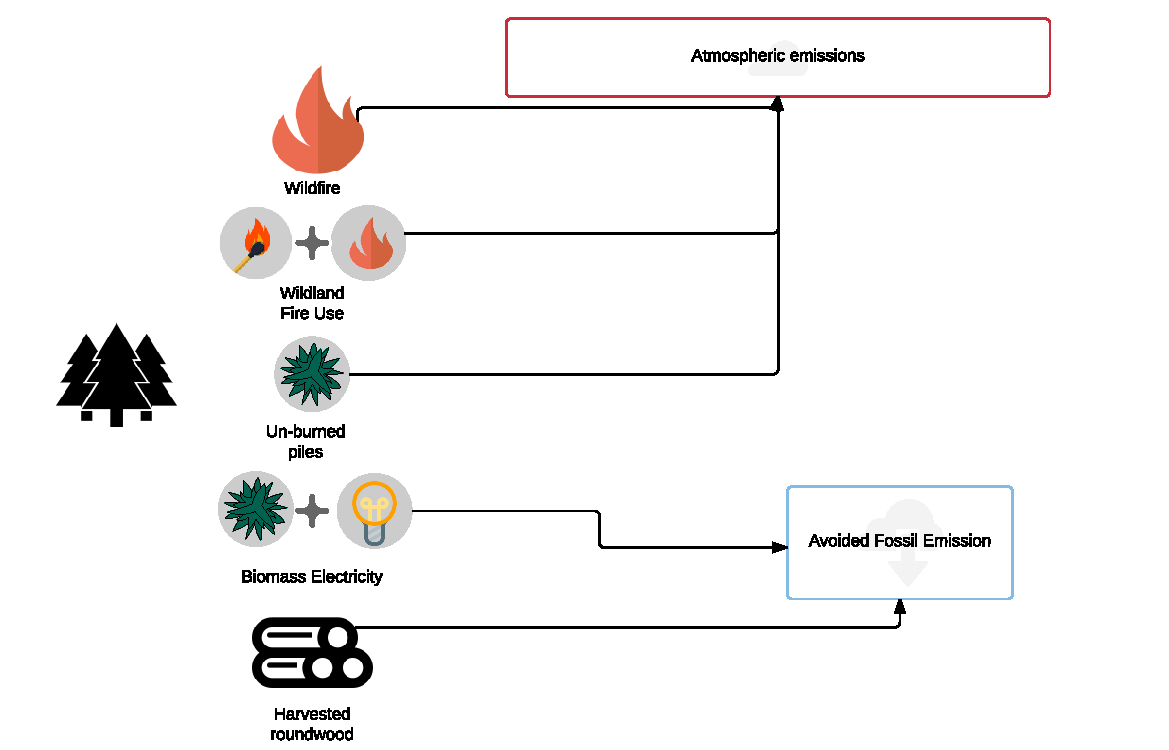
\includegraphics[width=0.75\textwidth]{./graphics/wood_fates.pdf}
\caption{Overview of the system. \label{fig:wood_fates}}
\end{figure}


Quantifying the climate effects of wood products and forest management residuals is
important to the development of the Forest Climate Plan (FCP)\footnote{The \href{http://www.fire.ca.gov/fcat/}{Forest Climate Action Team} (FCAT) was assembled in August of 2014 with the primary purpose of developing a Forest Carbon Plan by the end of 2016. FCAT is comprised of Executive level members from many of the State’s natural resources agencies, state and federal forest land managers, and other key partners directly or indirectly involved in California forestry. FCAT is under the leadership of CAL FIRE, Cal-EPA, and The Natural Resources Agency.} as well
as efforts underway by the California Board of Forestry and CalFire to
meet the intent of AB 1504 (2010)\footnote{\href{http://leginfo.legislature.ca.gov/faces/billTextClient.xhtml?bill_id=200920100AB1504}{AB-1504} Forest resources: carbon sequestration.(2009-2010)}. To inform these efforts, this
report provides estimates of the following :

\begin{enumerate}
\item GHG and SLCP emissions produced from the combustion or
decomposition of logging residuals.
\item GHG emissions reductions from the use of wood products harvested in
the state.
\end{enumerate}

Estimates are based on empirical data and reflect past forest
management activities. It is \textbf{critical} to note that the empirical
data used in this analysis reflect point-in-time measures that are
affected by a dynamic system of climate, growth, and mortality in
forests as well as macroeconomic and policy forces. To effective
manage forests for climate (and/or other) benefits, a process modeling
approach is necessary. This analysis may provide insight into
opportunities to more effectively utilize woody biomass residuals from
current forest management activities based on available historical
data.

Several steps are necessary to address the objective stated:

\begin{enumerate}
\item Estimate CO2 equivalent emissions from burning forest management
residuals using criteria pollutant and GHG emissions inventory
published by the California Air Resources Board (CARB)

\item Estimate the volume and fate of wood removed, left in the
forest, and burned as a result of direct anthropogenic management
activities.

\item Establish life-cycle displacement factors (DF) for all
utilized wood and apply DF to harvested wood to obtain an aggregate estimate.
\end{enumerate}

\subsubsection{Key Findings}
\label{sec:orgheadline1}

\begin{itemize}
\item Baseline emissions of GHG and SLCP emissions from burning of forest
management residuals can be estimated and should be considered in
any forest management emissions baseline.

\item Total emissions from pile burning of foreat management resulals
includine SLCP and GHG components extrapolated from CARB emissions
inventory is XXX MTCO2e

\item Harvested wood in California in 2012 resulted in avoided emissions of
4 MMTCO2e

\item Logging residuals not used in bioenergy production contributed
emissions of:
\begin{itemize}
\item XXX MMTCO2e resulting from anthropogenic burning of logging residuals

\item XXX MMTCO2e resulting from decomposition of loggin residuals left
unburned
\end{itemize}

\item Un-utilized slash from non-commercial management activities on
National Forest System lands contributed emissions of XXX MMTCO2e

\item Forest Inventory and Analysis re-sample data has been used in the
southeast to quantify removals resulting from non-commercial
management activity and could be used for this purpose in California

\item The \href{https://ssl.arb.ca.gov/pfirs/}{Prescribed Fire Information Reporting System} (PFIRS) may be a usefull tool in quantifying
emissions from pile burns and prescribed fire. However, at this time
it is not a requirement for California Air Quality Management
Districts to report emissions through this system, and thus it is not
comprehensive. It is a requirment that prescribed fires and pile
burns on National Forest System Lands are reported through PFIRS. It
is not possible at this point to associate burns in PFIRS with
commercial harvest activities.
\end{itemize}


\subsection{Estimating CO2 equivalent emissions from forest biomass burning}
\label{sec:orgheadline4}

\begin{figure}[htb]
\centering
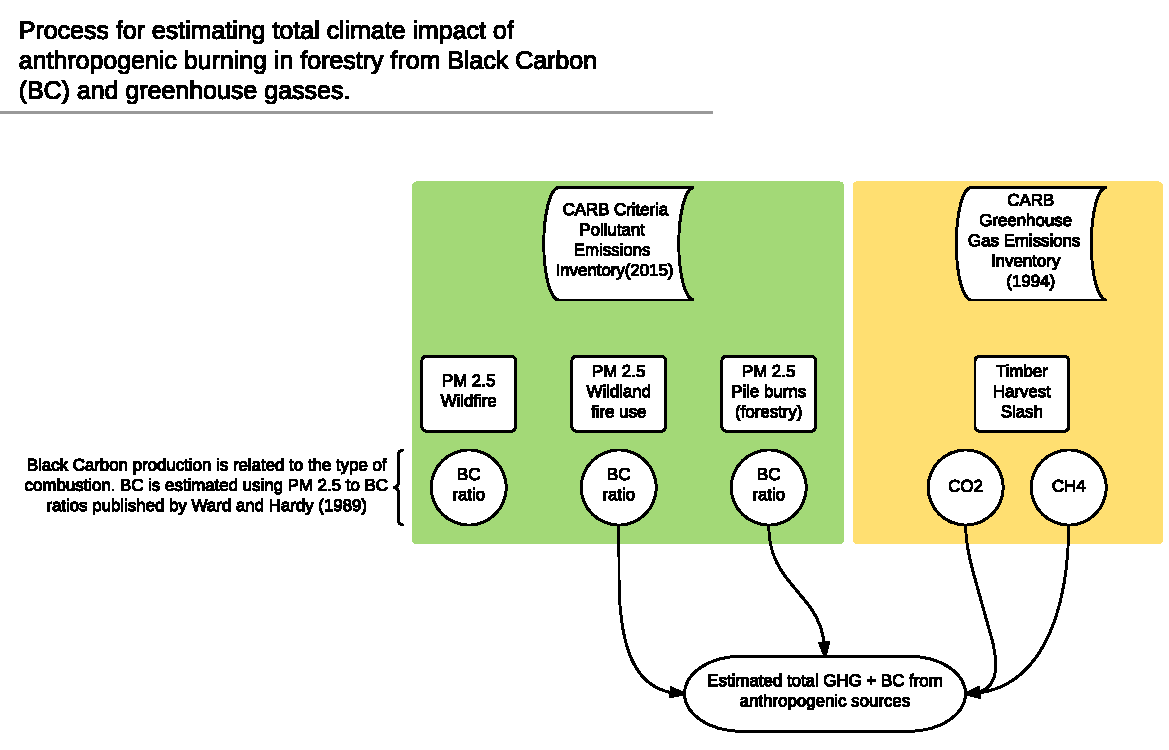
\includegraphics[width=0.75\textwidth]{./graphics/burning.pdf}
\caption{Data sources available from CARB for estimating GHG and SLCP emissions from forest management. \label{fig:wood_fates}}
\end{figure}


\subsubsection{Estimating black carbon emissions from biomass burning}
\label{sec:orgheadline3}

The California Air Resources Board (CARB) reports
emissions from forest biomass burning  in the most current
\href{http://www.arb.ca.gov/ei/ei.htm}{statewide emissions inventory}. The Criteria Air
Pollutant (CAP) emissions inventory and the Greenhouse Gas (GHG)
emissions inventory are both necessary sources for establishing
aggregate annual climate-forcing emissions. The GHG inventory captures
gasses with radiative forcing properties but does not capture elemental
carbon or black carbon (BC) emissions which have strong radiative
forcing properties. The \citet{CaliforniaAirResourcesBoard2015,CaliforniaAirResourcesBoard2016}
reports aggregate SLCP emissions from wildfire
(\texttt{80.52} MMTCO2e), and from prescribed fire
(\texttt{3.66} MMTCO2e). However, no reference in the
SLCP Strategy is made to the source of these estimates.

The California Air Resources Board has published
\href{http://www.arb.ca.gov/ei/emissiondata.htm}{criteria air pollutant
emissions estimates for 2015}. Particulate matter as reported in the
criteria air pollutant emissions inventory contains black carbon which
is a strong short lived climate pollutant.


\begin{table}[htb]
\centering
\begin{tabular}{rrrrrrl}
GWP\(_{\text{20}}\) & GWP\(\sigma_{\text{20}}\) & GWP\(_{\text{100}}\) & GWP\(\sigma_{\text{100}}\) & GWP\(_{\text{500}}\) & GWP\(\sigma_{\text{500}}\) & Source\\
\hline
2200.0 & 888.82 & 633.33 & 255.41 & 193.33 & 77.67 & Fuglestvedt2010\\
3200.0 &  & 900.0 &  &  &  & CaliforniaAirResourcesBoard2015\\
\end{tabular}
\caption{Range of GWP values for Black Carbon.}

\end{table}




CARB reports PM 2.5 emissions in tons/day. Annual emissions  as
reported by CARB are shown in

\begin{center}
\begin{tabular}{lr}
Source & PM 2.5 (t y\(^{\text{-1}}\))\\
\hline
ALL VEGETATION & 137630.15\\
FOREST MANAGEMENT & 5480.51\\
WILDLAND FIRE USE (WFU) & 6802.43\\
\end{tabular}

\end{center}

Black Carbon emissions
can be estimated from PM 2.5 emissions if the ratio of smoldering to
flaming combustion is known. \citet{Ward1989} provide estimates of
the ratio of smoldering to flaming combustion for a hand/machine piled
burns, prescribed natural fire and wildfire. BC is a fraction
of the Total Carbon (TC) component of PM 2.5. Thus BC is related to PM
2.5 by Eq. \eqref{eq-bc} :



\begin{align}
BC &= \left( PM_{2.5} \times F \times TC_f \times BC_f\right) + \left( PM_{2.5} \times S \times TC_s \times BC_s\right) \label{eq-bc} \\
\text{where:} \nonumber \\
BC &= \text{Black Carbon (mass units)} \nonumber \\
PM_{2.5} &= PM_{2.5} \text{ (mass units)} \nonumber \\
F &= \text{Percent of combustion in flaming phase} \nonumber \\
TC_f &= \text{Total Carbon fraction of } PM_{2.5} \text{ for flaming phase} \nonumber \\
BC_f &= \text{Black Carbon fraction of Total Carbon for flaming phase} \nonumber \\
S &= \text{Percent of combustion in smoldering phase} \nonumber \\
TC_s &= \text{Total Carbon fraction of } PM_{2.5} \text{ for smoldering phase} \nonumber \\
BC_s &= \text{Black Carbon fraction of Total Carbon for smoldering phase} \nonumber
\end{align}

Based on \citet{Ward1989} and \citet{Jenk1996} the following ratios are
used herein.

\begin{table}[htb]
\centering
\begin{tabular}{lrrrrrr}
Source & BC\(_{\text{f}}\) t\(^{\text{-1}}\) PM & TC\(_{\text{f}}^{\text{Cv}}\) t\(^{\text{-1}}\) PM & BC\(_{\text{f}}^{\text{Cv}}\) t\(^{\text{-1}}\) TC & BC\(_{\text{s}}\) t\(^{\text{-1}}\) PM 2.5 & TC\(_{\text{s}}^{\text{Cv}}\) t\(^{\text{-1}}\) PM & BC\(_{\text{s}}^{\text{Cv}}\) t\(^{\text{-1}}\) TC\\
\hline
Pile Burn & 0.046904 & 0.09 & 0.45 & 0.01624 & 0.01 & 0.49\\
Prescribed & 0.08016309 & 0.0733 & 0.5833 & 0.020944 & 0.08 & 0.29\\
Wildfire & 0.05870124 & 0.0867 & 0.4467 & 0.0228641 & 0.06 & 0.338\\
\end{tabular}
\caption{Factors used for calculating Black Carbon (BC) emissions from three primary combustion sources. BC is a fraction of Total Carbon (TC) which is a fraction of total PM 2.5. Coefficients of variation (C\(_{\text{v}}\)) are reported here as well.}

\end{table}



To arrive at a rough estimate of BC emissions based on PM2.5 the
following steps are taken

\begin{enumerate}
\item Determine the amount of PM2.5 produced in the flaming and smoldering
phases of combustion for each type (piles, prescribed,
wildfire). Ratios from \citet{Ward1989}, table 5 are used.
\item Define 1000 normal probability distributions using the coefficient
of variation from Table \ref{tab:bc_pmfor} the percent of PM2.5
comprised of carbonaceous material (TC) and percent of TC comprised
of black carbon (BC) give estimates and coefficient of variation
estimates provided by \citet{Ward1989}, tables 2 and 3.
\item Estimate annual BC emissions based on probability distributions
defined in 2.
\end{enumerate}

The following plot represents estimates of total BC emissions resulting
from combustion of biomass in the CARB CPE emissions categories
reflecting woody biomass combustion in wildfire, pile burning and
prescribed natural fire.

\begin{figure}[htb]
\centering
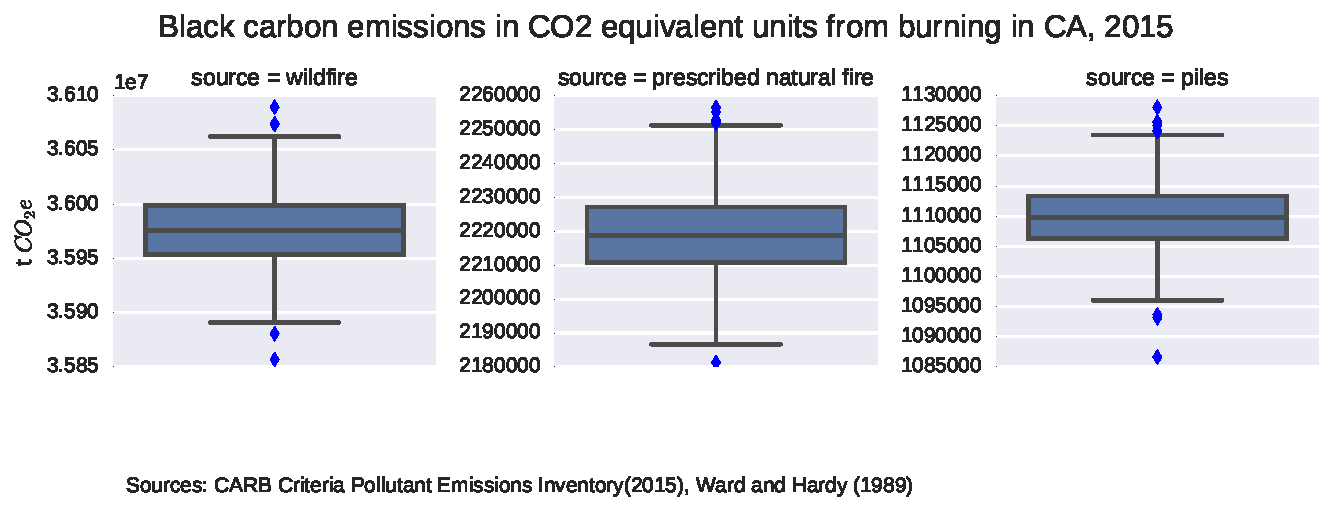
\includegraphics[width=\textwidth]{./graphics/bc_prob_gwp.pdf}
\caption{Short-lived climate pollution from open burning of biomass as reported by CARB criteria pollutant emissions inventory.}
\end{figure}

In addition the
\url{http://www.arb.ca.gov/cc/inventory/archive/tables/net_co2_flux_2007-11-19.pdf}
CARB 1994 greenhouse gas emissions inventory estimates emissions from
wildfire and slash burning through 2004 (Table \ref{arb_ghg_2004}).
\begin{center}
\begin{tabular}{lr}
Source Category & Average annual emissions 1994-2004 MMTCO\(_{\text{2e}}\)\\
\hline
Forest and rangeland fires & 2.0194\\
Timber harvest slash & 0.155266666666667\\
\end{tabular}

\end{center}


To arrive at an estimate of total emissions in 2015 from burning forest
management residuals in CO2 equivalent terms from published CARB
estimates we can combine the CO2 emissions reported for 2004 in the
LULUC Biodegradable Carbon Emissions and Sinks with black carbon
emissions extrapolated from the CARB Criteria Air Pollutant Emissions
inventory estimates. The time discrepancy between the 2004 and 2015 is
acknowledged as an irreconcilable source of uncertainty in this
estimation. Further model based estimation could be used to derive a
ratio of GHG to PM using the CONSUME model. This does however show that a baseline of
substantial emissions from forest management residuals has been reported
in CARB emissions inventories and should be recognized as a baseline
condition. We find that a rough estimate of CO2e emissions from pile
burning annual approaches 1 Mt CO2e.

\begin{center}
\begin{tabular}{rrl}
 & Mt CO2e & Source\\
\hline
0 & 0.17 & CO2 pile burning\\
1 & 0.99 & CO2e BC pile burning\\
2 & 1.16 & Total Mt CO2e\\
\end{tabular}

\end{center}

BC emissions in terms of CO2e has not been included in any GHG emissions
inventory published by CARB.



\subsection{Fate of harvested wood}
\label{sec:orgheadline12}
Wood harvested from California's forests is used in construction,
landscaping and consumer products. Residual streams from the
production of these wood products are used to generate elctricity and
heat and a protion if the residual goes to landfills or is left in the
woods as slash.

\subsubsection{Wood Displacement Factors}
\label{sec:orgheadline5}

In all of its applications, a range of other products can be used in place of wood. For example, in
residential construction, precast concrete and structural steel framing
are competitive alternatives to wood. The choice of materials used in
construction has a profound impact on GHG emissions from the
construction sector. This impact can be expressed as a displacement
factor (DF). A displacement factor quantifies the amount of emissions
reduction achieved per unit of wood used. A meta analysis conducted by \citep{Sathre2010} compared empirical analysis from 21 international studies and found an
average emissions reduction of 2.1 tons of carbon (3.9 t CO2e) per ton
of dry wood used. Studies ranged substantially around the average, the
authors found that the majority of published displacement factors ranged
between 1 and 3 tC/t dry wood. The displacement factors published in
\citep{Sathre2010} and used in this analysis include the
following sources emissions reduction:

\begin{enumerate}
\item \textbf{Reduced emissions from manufacturing:} Wood products require total
energy than than manufacturing most alternative materials.
\item \textbf{Avoided process emissions:} Wood-alternatives such as cement have
substantial CO2 emissions associated with production.
\item \textbf{Carbon storage in products:} Carbon in harvest wood was drawn from
the atmosphere through photosynthesis and will remain fixed through
the useful life of the wood product.
\item \textbf{Carbon storage in forests:} Forests producing wood continue to grow.
It is assumed that forests producing wood in California are managed
to sustain forest growth (not converted to non-forest land uses).
\item \textbf{Avoided fossil fuel emissions due to bioenergy substitution:}
Logging and milling residuals used to produce energy avoid emissions
from fossil energy sources in the energy sector.
\item \textbf{Carbon dynamics in landfills:} A fraction of carbon in wood
deposited in landfills post use remains in semi-permanent storage.
The remainder is converted to methane through biological
decomposition in the landfill. Capture and use of the methane as an
energy source, in turn reduces emissions from fossil energy sources.
\end{enumerate}

\subsubsection{Displacement Factors Applied to Timber Products Output}
\label{sec:orgheadline6}

To evaluate the climate impact of harvested wood in California I use
harvested roundwood estimates from the Timber Products Output (TPO)
database\footnote{Timber Products Output Reporting Tool \href{http://srsfia2.fs.fed.us/php/tpo_2009/tpo_rpa_int1.php}{\url{http://srsfia2.fs.fed.us/php/tpo_2009/tpo_rpa_int1.php}}}. I use two estimates of the DF applied
to the harvested wood reported in the TPO based on weather logging
residuals are used in bioenergy or left in the woods to decompse or
burn.

Figure \ref{fig:flow_chart} reflects the flow of wood
from Californias forest to its fate in-use and is the frame of
reference for the following analysis.

\begin{figure}[htb]
\centering
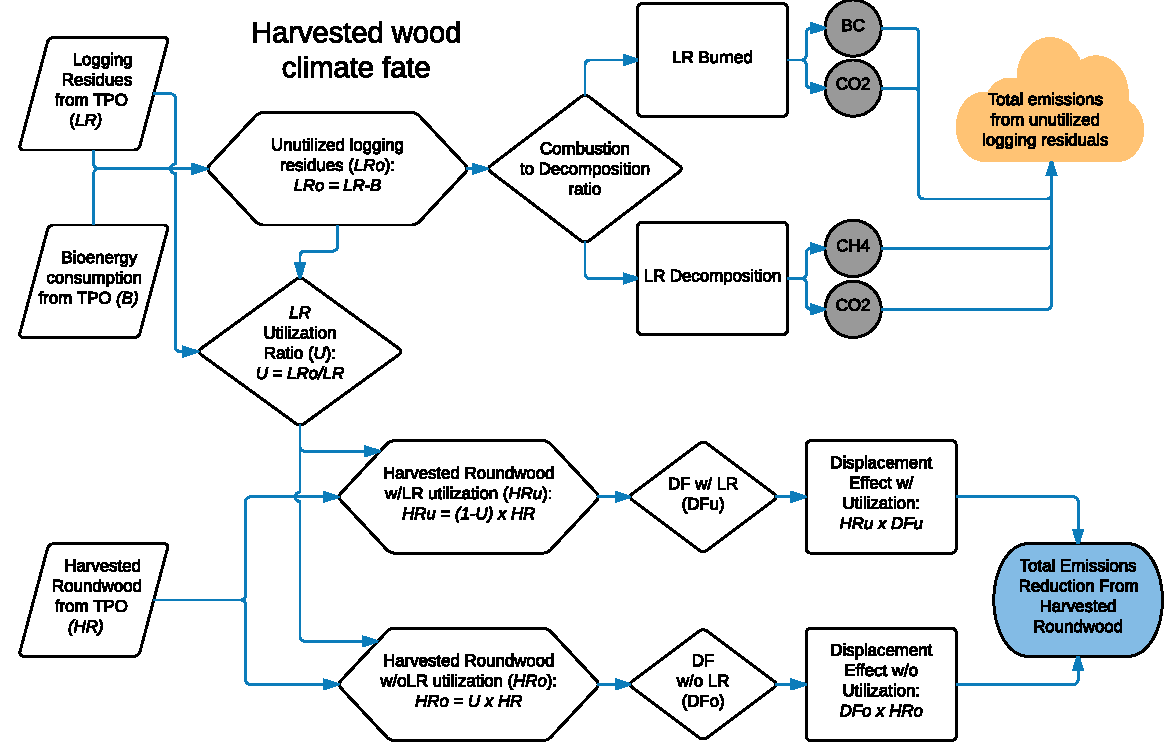
\includegraphics[width=0.75\textwidth]{./graphics/flow_chart.pdf}
\caption{Wood flows from commercial timber harvest in California \label{fig:flow_chart}}
\end{figure}

I use displacement factors reported by \cite{Sathre2010} applied to the
reported volumes from the TPO. The following references are used to
arrive at a displacement factor for harvested roundwood without
logging residue utilization.

\begin{center}
\begin{tabular}{lr}
reference & displacement factor\\
\hline
\citet{Eriksson2007} & 1.7\\
\citet{Eriksson2007} & 2.2\\
\citet{Salazar2009} & 4.9\\
\citet{Werner2005} & 1.7\\
\end{tabular}

\end{center}

I use an average of the DF reported here of \textbf{2.625} tCO2e/t finished
wood product. For harvested roundwood with logging residue utilization the following
studies are used.

\begin{center}
\begin{tabular}{lr}
reference & displacement factor\\
\hline
\citet{Eriksson2007} & 1.9\\
\citet{Eriksson2007} & 2.5\\
\citet{Gustavsson2006a} & 4\\
\citet{Gustavsson2006a} & 5.6\\
\citet{Gustavsson2006a} & 2.2\\
\citet{Gustavsson2006a} & 3.3\\
\citet{Pingoud2001} & 3.2\\
\end{tabular}

\end{center}

I use an average of the DF reported here of \textbf{3.243} tCO2e/t finished
wood product.

TPO is reported in terms of roundwood harvested for products. The
displacement factors presented in Sathre and O'Connonr are in terms of
tons of carbon in wood products. Therefore we must assume a milling
efficiency to convert TPO estimates to finished wood products. I assume
a milling efficiency of 0.5.

Further, TPO is reported in in cubic feet and the DF implies a mass
unit. To convert cubic meters to a mass unit we use the average wood
density of harvested volume in California weighted by species. Harvest
volume by species is reported in \citet{Mciver2012}. The resulting weighted average wood density used here is \textbf{27.94
lbs/cuft}.

McIver and Morgan report the percent of harvest used as bioenergy
feedstock. From personal communications with
\href{http://www.bber.umt.edu/staff/mciver.asp}{Chelsea McIver}, all bioenergy feedstock reported is sourced in-woods (ie, not mill
residues).

\begin{center}
\begin{tabular}{rrr}
 & year & bioenergy \% of harvest\\
\hline
0 & 2000 & 0.024\\
1 & 2006 & 0.036\\
2 & 2012 & 0.082\\
\end{tabular}

\end{center}

The TPO reports the total logging residues produced from the states
harvest.

\begin{center}
\begin{tabular}{rlrrr}
 & Ownership & Roundwood Products & Logging Residues & Year\\
\hline
0 & National Forest & 72.4 & 20.7 & 2012\\
1 & Other Public & 16.2 & 3.4 & 2012\\
2 & Forest Industry & 328.9 & 72.4 & 2012\\
3 & Other Private & 53 & 11.2 & 2012\\
4 & National Forest & 52.8 & 16.3 & 2006\\
5 & Other Public & 1.1 & 0.3 & 2006\\
6 & Forest Industry & 274.3 & 59.6 & 2006\\
7 & Other Private & 139.2 & 33.2 & 2006\\
8 & National Forest & 90.8 & 22.6 & 2000\\
9 & Other Public & 5.2 & 1.6 & 2000\\
10 & Forest Industry & 372.5 & 70.6 & 2000\\
11 & Other Private & 159.4 & 49.1 & 2000\\
12 & National Forest & 132.1 & 11.2 & 1994\\
13 & Other Public & 24.7 & 4.3 & 1994\\
14 & Forest Industry & 396.1 & 63.1 & 1994\\
15 & Other Private & 174.7 & 22.3 & 1994\\
\end{tabular}

\end{center}


In addition to the TPO, the California Board of Equalization (BOE
reports historical timber harvest.  Averaged over the years where both
sources report data, the BOE is 8\% less than TPO (Table \ref{tab:tpo_boe}). This is reasonable considering that:
\begin{enumerate}
\item BOE data may under-reported as there may be a financial incentive to reduce tax burden
\item BOE does not include volume harvested from native American tribal lands in the state
\end{enumerate}

\begin{longtable}{rrrr}
year & McIver, et. al. (2012) MMBF & BOE MMBF & BOE/M\&M\\
\hline
\endfirsthead
\multicolumn{4}{l}{Continued from previous page} \\
\hline

year & McIver, et. al. (2012) MMBF & BOE MMBF & BOE/M\&M \\

\hline
\endhead
\hline\multicolumn{4}{r}{Continued on next page} \\
\endfoot
\endlastfoot
\hline
1978 & 4606.0 & 4491 & 0.98\\
1979 & 4044.0 & 3991 & 0.99\\
1980 & 3478.0 & 3164 & 0.91\\
1981 & 2832.0 & 2672 & 0.94\\
1982 & 2488.0 & 2318 & 0.93\\
1983 & 3638.0 & 3358 & 0.92\\
1984 & 3701.0 & 3546 & 0.96\\
1985 & 4093.0 & 3818 & 0.93\\
1986 & 4416.0 & 4265 & 0.97\\
1987 & 4667.0 & 4500 & 0.96\\
1988 & 4847.0 & 4670 & 0.96\\
1989 & 4699.0 & 4424 & 0.94\\
1990 & 4264.0 & 4021 & 0.94\\
1991 & 3439.0 & 3195 & 0.93\\
1992 & 3192.0 & 2973 & 0.93\\
1993 & 3041.0 & 2871 & 0.94\\
1994 & 2814.0 & 2316 & 0.82\\
1995 & 2520.0 & 2306 & 0.92\\
1996 & 2515.0 & 2273 & 0.9\\
1997 & 2640.0 & 2400 & 0.91\\
1998 & 2420.0 & 2091 & 0.86\\
1999 & 2429.0 & 2144 & 0.88\\
2000 & 2244.0 & 1966 & 0.88\\
2001 & 1801.0 & 1603 & 0.89\\
2002 & 1691.73 & 1690 & 1.0\\
2003 & 1667.95 & 1663 & 1.0\\
2004 & 1704.0305 & 1706 & 1.0\\
2005 & 1738.5 & 1725 & 0.99\\
2006 & 1960.35 & 1631 & 0.83\\
2007 & 1759.6 & 1626 & 0.92\\
2008 & 1476.0745 & 1372 & 0.93\\
2009 & 911.19 & 805 & 0.88\\
2010 & 1302.38 & 1161 & 0.89\\
2011 & 1432.5 & 1288 & 0.9\\
2012 & 1421.3 & 1307 & 0.92\\
\caption{Total annual harvest reported by \citet{Mciver2012} and California Board of Equalization.}
\\
\end{longtable}

The BOE does not report harvest from tribal lands but the TPO does. By
TPO data, harvest from tribal lands averages 0.74\% of the total
annual harvest in the state for the 37 years of parallel data. For
this analysis we use TPO data and include tribal lands. 


\begin{longtable}{rrrrr}
year & State & Federal & Private & Tribal\\
\hline
\endfirsthead
\multicolumn{5}{l}{Continued from previous page} \\
\hline

year & State & Federal & Private & Tribal \\

\hline
\endhead
\hline\multicolumn{5}{r}{Continued on next page} \\
\endfoot
\endlastfoot
\hline
1947 & 0.0 & 0.0 & 569.85 & 0.0\\
1948 & 0.0 & 0.0 & 735.29 & 0.0\\
1949 & 0.0 & 0.0 & 698.53 & 0.0\\
1950 & 0.0 & 0.0 & 808.82 & 0.0\\
1951 & 0.0 & 0.0 & 900.74 & 0.0\\
1952 & 2.57 & 113.79 & 808.82 & 4.78\\
1953 & 3.31 & 117.65 & 977.94 & 2.76\\
1954 & 2.94 & 141.54 & 880.51 & 4.6\\
1955 & 2.57 & 191.73 & 906.25 & 6.07\\
1956 & 4.41 & 206.99 & 862.13 & 5.33\\
1957 & 4.96 & 170.59 & 801.47 & 6.62\\
1958 & 5.51 & 208.27 & 821.69 & 6.99\\
1959 & 4.96 & 279.6 & 788.6 & 9.19\\
1960 & 5.15 & 250.37 & 680.15 & 8.82\\
1961 & 5.33 & 259.74 & 707.72 & 10.11\\
1962 & 6.25 & 259.01 & 744.49 & 8.64\\
1963 & 4.04 & 311.76 & 678.31 & 9.93\\
1964 & 4.6 & 348.16 & 643.38 & 9.01\\
1965 & 5.7 & 363.05 & 591.91 & 9.74\\
1966 & 5.88 & 360.85 & 545.96 & 8.27\\
1967 & 6.43 & 355.51 & 562.5 & 7.54\\
1968 & 8.82 & 440.44 & 542.28 & 14.52\\
1969 & 7.35 & 372.61 & 529.41 & 9.93\\
1970 & 6.25 & 345.4 & 481.62 & 5.15\\
1971 & 7.17 & 383.09 & 476.1 & 12.87\\
1972 & 6.8 & 411.58 & 591.91 & 12.13\\
1973 & 6.07 & 371.69 & 516.54 & 9.38\\
1974 & 7.35 & 322.79 & 525.74 & 9.38\\
1975 & 6.43 & 287.87 & 498.16 & 3.31\\
1976 & 7.35 & 348.53 & 507.35 & 6.99\\
1977 & 5.15 & 323.35 & 544.12 & 6.99\\
1978 & 5.15 & 332.35 & 509.19 & 8.64\\
1979 & 4.78 & 321.32 & 417.28 & 8.82\\
1980 & 3.68 & 279.04 & 356.62 & 7.72\\
1981 & 2.76 & 201.65 & 316.18 & 4.04\\
1982 & 7.72 & 173.9 & 275.74 & 1.47\\
1983 & 7.9 & 313.42 & 347.43 & 2.57\\
1984 & 6.25 & 288.05 & 386.03 & 3.86\\
1985 & 6.62 & 339.52 & 406.25 & 0.92\\
1986 & 5.33 & 365.26 & 441.18 & 4.96\\
1987 & 7.72 & 364.89 & 485.29 & 7.54\\
1988 & 5.7 & 403.68 & 481.62 & 2.57\\
1989 & 6.8 & 373.53 & 483.46 & 2.02\\
1990 & 4.41 & 283.09 & 496.32 & 2.57\\
1991 & 6.99 & 248.35 & 376.84 & 4.41\\
1992 & 4.23 & 190.99 & 391.54 & 5.88\\
1993 & 6.25 & 137.32 & 415.44 & 2.39\\
1994 & 3.12 & 152.02 & 362.13 & 2.76\\
1995 & 7.35 & 101.1 & 354.78 & 2.94\\
1996 & 10.11 & 86.4 & 365.81 & 2.39\\
1997 & 8.64 & 101.65 & 375.0 & 2.76\\
1998 & 4.78 & 83.46 & 356.62 & 2.94\\
1999 & 0.0 & 97.24 & 349.26 & 0.0\\
2000 & 3.49 & 63.42 & 345.59 & 1.84\\
2001 & 2.94 & 56.07 & 272.06 & 1.84\\
2002 & 0.18 & 31.38 & 279.41 & 2.5\\
2003 & 0.18 & 28.85 & 277.57 & 3.29\\
2004 & 0.18 & 20.78 & 292.28 & 3.05\\
2005 & 0.18 & 43.66 & 275.74 & 1.95\\
2006 & 0.74 & 41.61 & 318.01 & 2.37\\
2007 & 0.18 & 58.57 & 264.71 & 3.55\\
2008 & 0.18 & 37.7 & 233.46 & 2.48\\
2009 & 0.18 & 30.37 & 136.95 & 0.72\\
2010 & 0.18 & 49.89 & 189.34 & 1.79\\
2011 & 0.18 & 55.42 & 207.72 & 2.1\\
2012 & 5.13 & 37.39 & 218.75 & 1.49\\
\caption{Annual harvest by ownership from \citet{Mciver2012} (MCF)}
\\
\end{longtable}

To use the TPO data to estimate emissions reductions using the DF we apply a
conversion factor of \textbf{5.44} MCF/MMBF. This is an approximation as the
actual sawlog conversion factor varies with the log size which, on
average over time has changed.  


The ratio of harvested volume to which we can apply a displacement
factor reflecting bioenergy use of logging residuals can be calculated
based on the ratio of reported consumption of logging residuals in
bioenergy by \citeauthor{Mciver2012} to the total logging residuals reported
in the TPO. \citeauthor{Mciver2012} report bioenergy consumption from 2000
forward. For years previous, we use the average bioenergy consumption
from 2000 -- 2012. These results assume bioenergy consumption
throughout the reporting years. Bioenergy use of residuals did not
begin until the late 1970. Further analysis is necessary to modify
these results to reflect the development of the bioenergy industry.

To calculate the total emissions reduction resulting from California's
timber harvest, we apply the appropriate displacement factor (with or
without logging residual utilization) to the commensurate fraction of
harvested roundwood. The results are shown in the following chart.

\begin{figure}[htb]
\centering
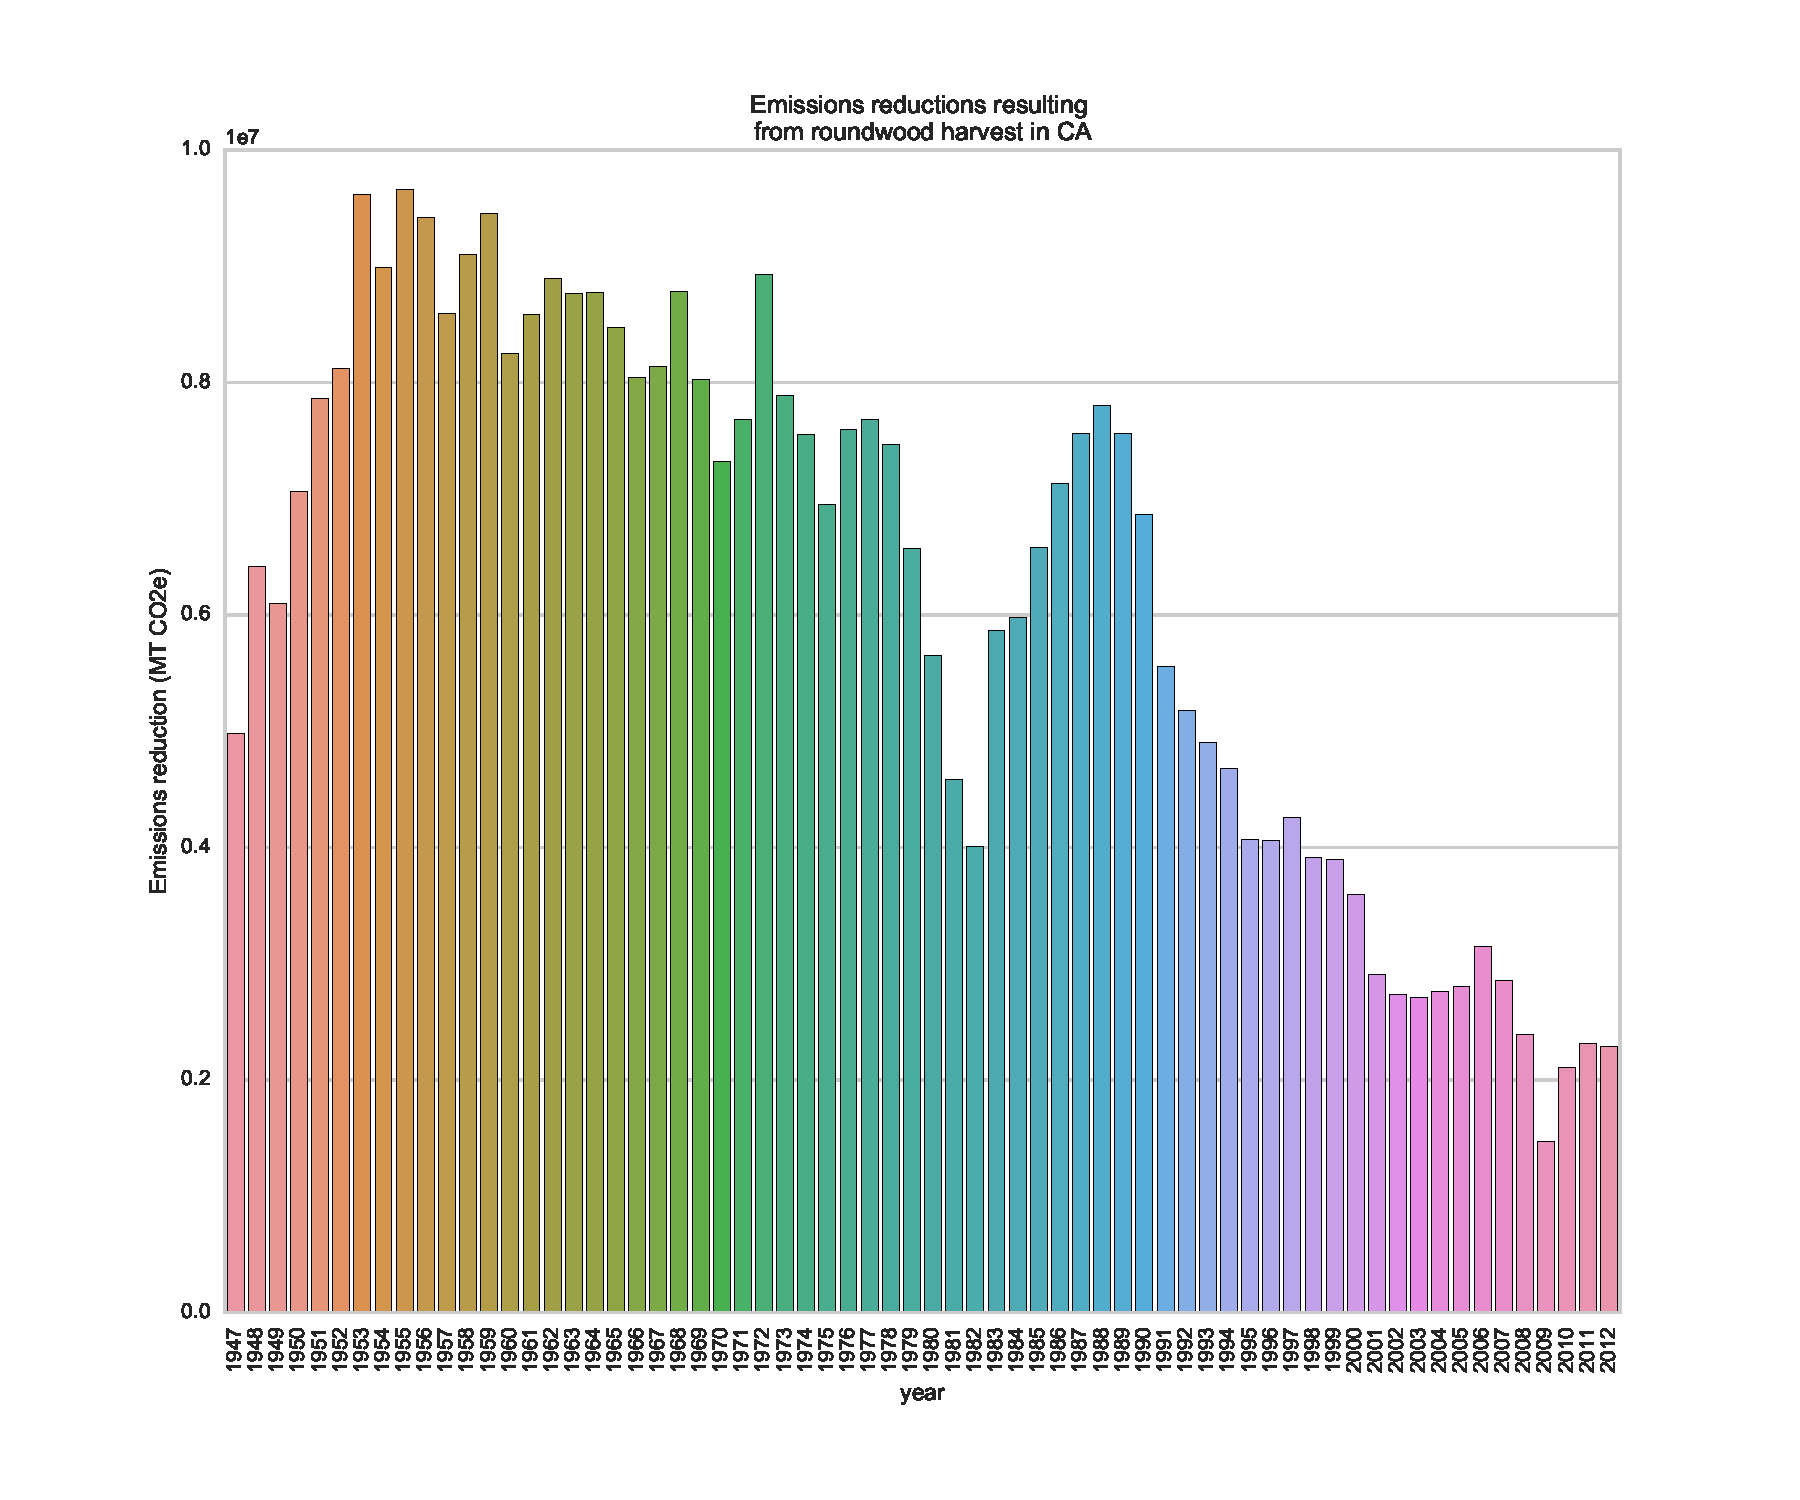
\includegraphics[width=\textwidth]{./graphics/ann_hh_em_reduc.pdf}
\caption{Historical emissions reductions resulting from harvested roundwood using displacement factors from \citep{Sathre2010} applied to TPO data.}
\end{figure}

Contribution of the varios ownership categories to the aggregate is
shown in Figure \ref{em_reduc_own}.

\begin{figure}[htb]
\centering
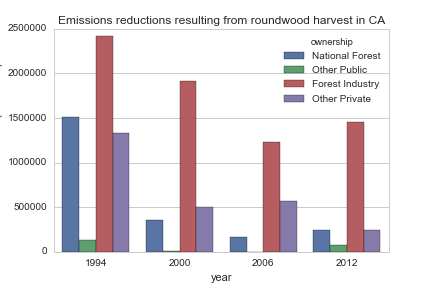
\includegraphics[width=.9\linewidth]{./graphics/harv_em_reductions.png}
\caption{\label{fig:orgparagraph1}
Historical emissions reductions by ownership for selected years resulting from harvested roundwood using displacement factors from \citep{Sathre2010} applied to TPO data.}
\end{figure}

\subsubsection{Emissions from un-utilized logging residues}
\label{sec:orgheadline8}

From logging residuals not used in bioenergy, emmisions are produced
from combustion of or from biological decomposition of the
material over time. To calculate the ratio of burned to decompsed
logging residues I begin with the CARB estimate of PM2.5 produced from
forest management. \#\#\#\# Estimate biomass from PM2.5 To estimate total
biomass from PM2.5 I assume 90\% consumption of biomass in piles and use
the relationship of pile tonnage to PM emissions calculated using the
\href{http://depts.washington.edu/nwfire/piles/}{Piled Fuels Biomass and Emissions Calculator} provided by the Washington State Department of
Natural Resources. This calculator is based on the \href{http://www.fs.fed.us/pnw/fera/research/smoke/consume/index.shtml}{Consume} fire behavior model published by the US Forest Service.

\begin{center}
\begin{tabular}{rrlrr}
 & YEAR & EICSOUN & Annual PM 2.5(t) & Biomass (BDT)\\
\hline
0 & 2000 & FOREST MANAGEMENT & 5474.31 & 901120\\
1 & 2005 & FOREST MANAGEMENT & 5474.31 & 901120\\
2 & 2010 & FOREST MANAGEMENT & 5474.31 & 901120\\
3 & 2012 & FOREST MANAGEMENT & 5477.3 & 901613\\
4 & 2015 & FOREST MANAGEMENT & 5480.51 & 902142\\
\end{tabular}

\end{center}

Total emissions resulting from pile burned forest management residuals
can then be derived for the two greenhouse gasses produced from pile
burning (CO2, CH4) and from BC:

\begin{center}
\begin{tabular}{rrlrrrr}
 & Year & Emissions source & CO2 (t) & CH4 (tCO2e) & BC (tCO2e) & Pile Burn (tCO2e)\\
\hline
0 & 2000 & FOREST MANAGEMENT & 1.34928\,(+06) & 127280 & 248255 & 1.72481\,(+06)\\
1 & 2005 & FOREST MANAGEMENT & 1.34928\,(+06) & 127280 & 248255 & 1.72481\,(+06)\\
2 & 2010 & FOREST MANAGEMENT & 1.34928\,(+06) & 127280 & 248255 & 1.72481\,(+06)\\
3 & 2012 & FOREST MANAGEMENT & 1.35002\,(+06) & 127349 & 248391 & 1.72576\,(+06)\\
4 & 2015 & FOREST MANAGEMENT & 1.35081\,(+06) & 127424 & 248536 & 1.72677\,(+06)\\
\end{tabular}

\end{center}

\begin{enumerate}
\item Emissions from decomposition of un-utilized forest management residuals
\label{sec:orgheadline7}

Un-utilized residual biomass not consumed in pile burns decomposes over
time resulting in emission of methane and carbon dioxide. To provide a
full picture of the emissions from residual material produced from
commercial timber harvesting in California, decomposition of unutilized
logging residuals left on-site that are not burned must be accounted
for. To establish the fraction of logging residue that is left to
decompose, residues burned and used in bioenergy are subtracted from the
total reported by the TPO:

\begin{align*}
LR_d &= LR - LR_{piles} - LR_{bio} \\
\text{where:}\\
LR_d &= \text{Logging residuals subject to anerobic decomposition} \\
LR &= \text{Total logging rsiduals reported by TPO}\\
LR_{piles} &= \text{Logging residues combusted in anthropogenic pile burns}\\
LR_{bio} &= \text{Logging residues used to produce bioenergy}
\end{align*}
To calculate the GHG emissions from decomposition of piles we use the
following equation.

\begin{align*}
CO_2e_{decomp} &= \left(LR_d \times C_{LR} \times CO2_{ratio} \right) + \left(LR_d \times C_{LR} \times CH_4_{ratio}\times GWP_{CH_4}\right)\\
\text{where:}\\
CO_2e_{decomp} &= \text{Carbon dioxide equivalent emissions from decomposition of logging slash}\\
C_{LR} &= \text{Carbon fraction of biomass: 0.5}\\
CO2_{ratio} &= \text{Fraction of carbon released as } CO_2\text{: 0.61}\\
CH_4_{ratio} &= \text{Fraction of carbon released as } CH_4\text{: 0.09}\\
GWP_{CH_4} &= \text{Global warming potential of methane: 56}
\end{align*}
\end{enumerate}

\subsubsection{Emissions from non-commercial management residuals}
\label{sec:orgheadline10}

/Note: Residues from non-commercial management activities are assumed to
be small in comparison with logging residues. In addition, there is
presently no empirical data available. As such, estimating these volumes
has not been prioritied. I have attempted to provide an estimate for
public lands in the National Forest System./

The TPO in California does not report wood volume produced from
non-commercial management activities. This includes management
activities such as pre-commercial thinning, sanitation thinning, and
fuels reduction thinning. To estimate the volume of material produced
from these activities we use the following sources:

\begin{enumerate}
\item \textbf{Public lands:} The USFS Forest Service Activity Tracking System
(FACTS) reports management activities conducted on National Forest
System Lands. To ensure estimates of biomass volume using FACTS are
not duplicative of reported volume in the TPO a series of filters are
applied to the FACTS attributes to identify only non-commercial
management activities.
\item \textbf{Private industrial timber lands:} CalFIRE's
\href{http://www.calfire.ca.gov/resource_mgt/resource_mgt_forestpractice_gis}{Forest
Practice Geographical Information System}. \textbf{TODO}
\end{enumerate}

\begin{enumerate}
\item Forest Service Activity Tracking System (FACTS)
\label{sec:orgheadline9}

Data from TPO does not account for forest management activities that do
not result in commercial products (timber sales, biomass sales). The
USFS
\href{http://data.fs.usda.gov/geodata/edw/datasets.php?dsetParent=Activities}{reports}
Hazardous Fuels Treatment (HFT) activities as well as Timber Sales (TS)
derived from the FACTS database. I use these two data sets to estimate
the number of acres treated that did not produce commercial material
(sawlogs or biomass) and where burning was not used. The first step is
to eliminate all treatments in the HFT data set that included timber
sales. I accomplish this by eliminating all rows in the HFT data set
that have identical \texttt{FACTS\_ID} fields in the TS dataset. I further
filter the HFT dataset by removing any planned but not executed
treatments (\texttt{nbr\_units1 >0} below -- \texttt{nbr\_units1} references
\texttt{NBR\_UNITS\_ACCOMPLISHED} in the USFS dataset, see metadata for HFT
\href{http://data.fs.usda.gov/geodata/edw/edw_resources/meta/S_USA.Activity_HazFuelTrt_PL.xml}{here}),
and use text matching in the 'ACTIVITY' and 'METHOD' fields to remove
any rows that contain reference to 'burning' or 'fire'. Finally, we
remove all rows that that reference 'Biomass' in the method category as
it is assumed that this means material was removed for bioenergy.I use a
range of 10-35 BDT/acre to convert acres reported in FACTS to volume.
The following table presents descriptive statistics for estimates of
residual unutilized wood biomass on an annual basis in million cubic
feet.

\begin{center}
\begin{tabular}{lrrrrr}
 & nf$\backslash$\(_{\text{n}}\) & nf$\backslash$\(_{\text{lr}}\) & opriv$\backslash$\(_{\text{lr}}\) & fi$\backslash$\(_{\text{lr}}\) & opub$\backslash$\(_{\text{lr}}\)\\
\hline
count & 11 & 4 & 4 & 4 & 4\\
mean & 12.0194 & 17.7 & 28.95 & 66.425 & 2.4\\
std & 4.68948 & 5.07346 & 16.1593 & 6.07639 & 1.79444\\
min & 2.37421 & 11.2 & 11.2 & 59.6 & 0.3\\
25\% & 8.92407 & 15.025 & 19.525 & 62.225 & 1.275\\
50\% & 13.3557 & 18.5 & 27.75 & 66.85 & 2.5\\
75\% & 14.5349 & 21.175 & 37.175 & 71.05 & 3.625\\
max & 17.8532 & 22.6 & 49.1 & 72.4 & 4.3\\
\end{tabular}

\end{center}
\end{enumerate}



\subsubsection{Disposition wood harvested in California.}
\label{sec:orgheadline11}

Harvested wood from California's forests is fractionated through harvest and processing and use into several categories for which the time horizon for return of carbon in biomass to the atmosphere can vary widely:

\begin{description}
\item[{Logging Residuals}] Tops, limbs and sub-merchantable material produced from harvest activities in the woods
\item[{Processing (mill) residuals}] Sawdust, shavings, bark and off cuts from primary and secondary manufacturing.
\item[{Construction debris}] Fraction of finished wood from finished products that is left from construction or integration into its final use.
\item[{Demolition}] Wood used in construction that has reached the end of its useful life.
\end{description}

Each category has multiple potential fates which can greatly influence the net emissions impact attributable to the initial forest management activity.  The fate of each of these pools is determined by a political and economic system which is highly dynamic. To understand how policy decisions will impact the fate and subsequent climate impact of harvested wood products, a detailed process model is necessary. To provide a rough estimate of the fate of annual round-wood harvest historically, we must use historical volumes and and apply what we know about milling efficiency improvements, logging utilization rates, and construction use efficiency. 

According to \citet{Morgan} logging residues produced from sawlog harvest can be estimated using a factor of 0.0302 (+/-.0123 @95\%CI) times the total cubic sawlog volume delivered to a mill. Unfortunately we cannot say how logging residue production has changed over time in California.  \citet{Simmons2014} found that logging utilization has decreased in Idaho from 1990 to 2011 by 72\%. For the purposed of this analysis we will assume that similar changes have occurred in California timber harvesting. We then estimate a logging residue production factor for years before 1990 based on the following equation wherein we assume 1990 residue ration for all years prior:


\begin{align*}
V\llap{--}lr_{x} = V\llap{--}rw_{x}\left(\eta_{04}+\left(\eta_{o4}\eta_\Delta\right)\right)\\
\text{Where:}\\
V\llap{--}rw_{x} = \text{Rundwood volume harvested in year }x\\
\eta_{04} = \mathcal{N}(0.0302,0.0123) \text{ ratio of logging residues to roundwood harvested in CA, 2004}\\
\eta_\Delta = 0.72 \text{ (percent change in efficiency over time period)}\\
\end{align*}

For logging residue production factors for years between 1990 and 2004 we calculate logging residues as a function of the percent change in logging residual rations estimated for Idaho from \citet{Simmons2014} applied to the known logging residual ratio reported by \citet{Morgan}. To reflect the uncertainty in the estimate provided by \citet{Morgan}, we calculate the logging residual using a randomly selected value from a normal probability distribution defined by the estimate and upper and lower bounds of the 95\% confidence interval provided:


\begin{align*}
V\llap{--}lr_{x} = V\llap{--}rw_{x}\left(\eta_{04}+ \left(\eta_{04}\left(\left(Y_1-x\right)\frac{\eta_\Delta}{Y_\Delta}\right)\right)\right)\\
\text{Where:}\\
V\llap{--}rw_{x} = \text{Rundwood volume harvested in year }x\\
\eta_{04} = \mathcal{N}(0.0302,0.0123) \text{ ratio of logging residues to roundwood harvested in CA, 2004}\\
Y_1 = 2004 \text{ (year for which logging residual estimate available for CA)} \\
x = \text{year for which logging residues are calculated}\\
\eta_\Delta = 0.72 \text{ (percent change in logging residue ratio over time period)}\\
Y_\Delta = 21\text{ (number of years over which logging residue ratio decreased)}
\end{align*}

Logging residual volume in years following 2004 are calculated as follows:

\begin{align*}
V\llap{--}lr_{x} = V\llap{--}rw_{x}\left(\eta_{04}- \left(\eta_{04}\left(\left(x-Y_1\right)\frac{\eta_\Delta}{Y_\Delta}\right)\right)\right)\\
\text{Where:}\\
V\llap{--}rw_{x} = \text{Rundwood volume harvested in year }x\\
\eta_{04} = \mathcal{N}(0.0302,0.0123) \text{ ratio of logging residues to roundwood harvested in CA, 2004}\\
Y_1 = 2004 \text{ (year for which logging residual estimate available for CA)} \\
x = \text{year for which logging residues are calculated}\\
\eta_\Delta = 0.72 \text{ (percent change in logging residue ratio over time period)}\\
Y_\Delta = 21\text{ (number of years over which logging residue ratio decreased)}
\end{align*}


Milling efficiency has increased roughly 14\% in California in the period between 1970 and 2006 \citet{Keegan2010}. For this analysis we assume a continuous improvement such that for years prior to 1970, milling efficiency in year \(x\) is calculated as:


\begin{align*}
V\llap{--}mr_{x} = V\llap{--}rw_{x} \left(\eta_{70}-\left((Y_1-x)\frac{\eta_\Delta}{Y_\Delta}\right\right)\\
\text{Where:}\\
V\llap{--}rw_{x} = \text{Rundwood volume harvested in year }x\\
\eta_{70} = 0.42 \text{ (milling efficiency in 1970)}\\
Y_1 = 1970 \text{ (earliest year mill efficiency available for)} \\
x = \text{year for which milling residues are calculated}\\
\eta_\Delta = 0.06\text{ (increase in milling efficiency from 1970-2011)}\\
Y_\Delta = 41\text{ (number of years overwhihc milling efficiency increased)}
\end{align*}

For years after 1970, milling efficiency for year \(x\) is calculated as:

\begin{align*}
V\llap{--}mr_{x} = V\llap{--}rw_{x} \left(\eta_{70}+\left((x-Y_1)\frac{\eta_\Delta}{Y_\Delta}\right\right)\\
\text{Where:}\\
V\llap{--}rw_{x} = \text{Rundwood volume harvested in year }x\\
\eta_{70} = 0.42 \text{ (milling efficiency in 1970)}\\
Y_1 = 1970 \text{ (earliest year mill efficiency available for)} \\
x = \text{year for which milling residues are calculated}\\
\eta_\Delta = 0.06\text{ (increase in milling efficiency from 1970-2011)}\\
Y_\Delta = 41\text{ (number of years overwhihc milling efficiency increased)}
\end{align*}


To estimate annualized construction and demolition material, we use ratios of finished wood products to construction debris and demolition debris referenced in \citet{McKeever2004}. This data is sparse and should be considered unreliable for years other than those for which it is reported in  \citeauthor{McKeever2004}. 

Construction debris was estimated in 2002 as approximately 15\% of total wood used in construction. Demolition debris from wood produced annually from wood grown on California forestland is outside of the scope of this report.


Table \ref{tab:me_and_lr} presents annualized estimates of logging and milling residuals, finished lumber, and construction debris based on BOE roundwood harvest volumes:

\begin{longtable}{rrrrrr}
Year & Total RW & LR & MR & FL & CD\\
\hline
\endfirsthead
\multicolumn{6}{l}{Continued from previous page} \\
\hline

Year & Total RW & LR & MR & FL & CD \\

\hline
\endhead
\hline\multicolumn{6}{r}{Continued on next page} \\
\endfoot
\endlastfoot
\hline
1978 & 825.551 & 59.3257 & 356.397 & 469.155 & 70.3732\\
1979 & 733.64 & 57.916 & 317.791 & 415.848 & 62.3773\\
1980 & 581.618 & 24.5204 & 252.791 & 328.827 & 49.324\\
1981 & 491.176 & 19.9015 & 214.201 & 276.976 & 41.5463\\
1982 & 426.103 & 28.368 & 186.446 & 239.657 & 35.9485\\
1983 & 617.279 & 23.1466 & 271.001 & 346.279 & 51.9418\\
1984 & 651.838 & 45.2246 & 287.127 & 364.711 & 54.7067\\
1985 & 701.838 & 15.3171 & 310.178 & 391.66 & 58.749\\
1986 & 784.007 & 66.4807 & 347.64 & 436.367 & 65.4551\\
1987 & 827.206 & 42.6001 & 368.006 & 459.2 & 68.88\\
1988 & 858.456 & 44.6082 & 383.164 & 475.291 & 71.2937\\
1989 & 813.235 & 76.8586 & 364.171 & 449.065 & 67.3597\\
1990 & 739.154 & 24.9964 & 332.079 & 407.076 & 61.0614\\
1991 & 587.316 & 28.9753 & 264.722 & 322.594 & 48.3891\\
1992 & 546.507 & 36.5019 & 247.128 & 299.379 & 44.9069\\
1993 & 527.757 & 23.3591 & 239.422 & 288.336 & 43.2504\\
1994 & 425.735 & 17.556 & 193.761 & 231.974 & 34.7961\\
1995 & 423.897 & 13.8504 & 193.545 & 230.352 & 34.5528\\
1996 & 417.831 & 8.74999 & 191.387 & 226.444 & 33.9666\\
1997 & 441.176 & 18.8119 & 202.726 & 238.451 & 35.7676\\
1998 & 384.375 & 12.8452 & 177.188 & 207.188 & 31.0781\\
1999 & 394.118 & 9.30322 & 182.255 & 211.862 & 31.7793\\
2000 & 361.397 & 13.1765 & 167.653 & 193.744 & 29.0616\\
2001 & 294.669 & 13.017 & 137.129 & 157.54 & 23.631\\
2002 & 310.662 & 7.25874 & 145.026 & 165.636 & 24.8454\\
2003 & 305.699 & 17.5243 & 143.156 & 162.542 & 24.3813\\
2004 & 313.603 & 8.57598 & 147.317 & 166.286 & 24.9429\\
2005 & 317.096 & 10.0085 & 149.422 & 167.674 & 25.1511\\
2006 & 299.816 & 9.0422 & 141.718 & 158.098 & 23.7147\\
2007 & 298.897 & 9.84822 & 141.721 & 157.176 & 23.5764\\
2008 & 252.206 & 9.86629 & 119.952 & 132.254 & 19.8381\\
2009 & 147.978 & 4.56935 & 70.5963 & 77.3816 & 11.6072\\
2010 & 213.419 & 1.37236 & 102.129 & 111.29 & 16.6935\\
2011 & 236.765 & 3.31091 & 113.647 & 123.118 & 18.4676\\
2012 & 240.257 & 7.77596 & 115.675 & 124.582 & 18.6873\\
2013 & 302.39 & 6.04001 & 146.032 & 156.358 & 23.4536\\
2014 & 269.485 & 9.0448 & 130.536 & 138.949 & 20.8424\\
\caption{Annualized logging and mill residual estimates based on BOE harvest volumes in Million Cubic Feet (MCF). RW:Roundwood harvested, LR: Logging residues, MR: Mill Residues, FL: Finished Lumber, CD: Construction Debris}
\\
\end{longtable}




\subsection{Further questions}
\label{sec:orgheadline13}

This analysis is a first step towards a broader analysis of the
climate impacts of harvested wood in California. The following are key
questions which follow from this analysis.
\subsection{References}
\label{sec:orgheadline14}
\bibliographystyle{IEEEtranSN}
\bibliography{fcat}
\end{document}